\documentclass{article}

% 导入中文宏包
\usepackage{ctex}
\usepackage{caption}
\usepackage{array}
\usepackage{hyperref}

% 设置标题、作者和日期
\title{Latex文档编辑与版本控制(Git)的初步了解}
\author{23020007073  刘畅}

% 设置页面边距
\usepackage{graphicx}
\usepackage{geometry}
\geometry{a4paper, left=2cm, right=2cm, top=3cm, bottom=4cm}

\begin{document}
	
	% 生成标题、作者和日期
	\maketitle
	
	% 心得报告正文
	\section{实验目的}
	本次课程讲授了版本控制(Git)与Latex文档编辑的使用,通过相应的学习熟悉这类快捷工具的使用
	
	\section{练习内容}
	\subsection{Latex学习例子10个}
	1. \verb|\verb命令里面||里面可以放入想表示的指令,这样它就会以文本的方式输出|
	
	2.begin[]和end[]可以构成环境,在里面可以编写内容。
	\begin{verbatim}
		begin[itemize]和end[itemize]构成无序列表,begin[enumerate]和end[enumerate]构成有序列表
		下面是例子:
	\end{verbatim}
	
		\begin{enumerate}
		\item 有序列表
	\end{enumerate}%有序列表,指有序号
	
	\begin{itemize}
		\item 无序列表
	\end{itemize}%有序列表,指有序号
	
	3. \verb|includegraphics[width=\textwidth]{}|该命令可以用来引入图片
	\begin{figure}
		\centering % 使图片居中
		\includegraphics[width=\textwidth]{"tupian.jpg"}
		\caption{这是样例3的图片。} % 图片的标题
		\label{fig:example} % 为图片设置标签,以便引用
	\end{figure}
	
	4.\begin{verbatim}
		\chapter{} 章节题目
		\section{} 标题
		\subsection{} 小部分
		\subsubsection{}更小的部分  从上往下层级依次细化
	\end{verbatim}
	
	5.\verb|\newline的功能是换行,可以使用 \newline 命令来实现换行。这个命令会将当前位置设置为新的一行|
	这便是用newline换新的一行\newline 
	
	6.\verb|\usepackage{}可以用来引入宏宝或者设置字体编码下面是几个例子|\begin{verbatim}
		\usepackage{amsmath}         % 数学公式
		\usepackage[utf8]{inputenc}  % 设置输入编码
		\usepackage{hyperref}        % 超链接
	\end{verbatim}
	
	7.\verb|创建表格的命令\hline|
	
	\begin{tabular}{|l|c|r|}
		\hline
		C1 & C2 & C3 \\
		\hline
		L & C & R \\
		\hline
	\end{tabular}
	\newline
	
	8.\verb|在公式中可以使用\color{options}{math}来调用颜色命令,第一个参数为颜色,第二个参数为公式或文本内容.|
	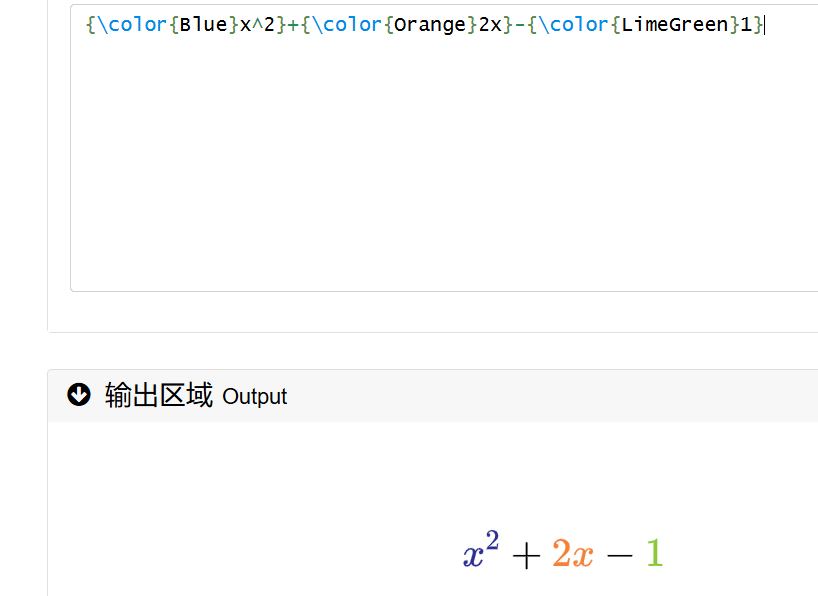
\includegraphics[width=\textwidth]{yanse.png}
	
	9.
	\verb|\textbf{}是加粗,\textit{}是倾斜,\underline{}是加下划线|
	
	This is \textbf{textbf}, this is \textit{textit}, and this is \underline{underline}.
	
	10.
	\title{Title} \verb|\title是加题目|
	
	\author{Author}\verb|\author是加作者|
	
	\date{Date}\verb|\date|是加日期|
	
	
	
	
	\subsection{Git学习例子10个}
	1.初始化新仓库:git init
	\noindent
	\begin{minipage}{\linewidth}
		\centering
		% 插入图片
		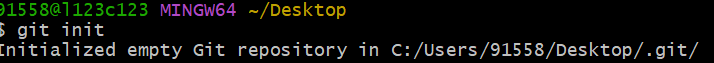
\includegraphics[width=0.5\linewidth]{init.png}
		% 图片标题
		\captionof{figure}{初始化新仓库}
		\label{fig:example}
	\end{minipage}
	
	
	2.配置开发者用户名:
	\noindent
	\begin{minipage}{\linewidth}
		\centering
		% 插入图片
		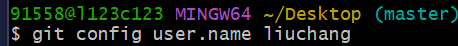
\includegraphics[width=0.5\linewidth]{name.png}
	\end{minipage}
	
	3.配置开发者邮箱:
	
	\noindent
	\begin{minipage}{\linewidth}
		\centering
		% 插入图片
		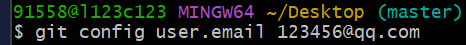
\includegraphics[width=0.5\linewidth]{email.png}
	\end{minipage}
	
	4.在处理文档时,一般创建分支来隔离开发工作:git branch
	\noindent
	\begin{minipage}{\linewidth}
		\centering
		% 插入图片
		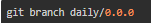
\includegraphics[width=0.5\linewidth]{daily.png}
		% 图片标题
		\captionof{figure}{创建分支}
		\label{fig:example}
	\end{minipage}
	
	5.切换分支:git checkout
	
	\noindent
	\begin{minipage}{\linewidth}
		\centering
		% 插入图片
		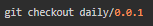
\includegraphics[width=0.5\linewidth]{checkout.png}
	\end{minipage}
	
	6.添加文件变动到暂存区:git add
	
	\noindent
	\begin{minipage}{\linewidth}
		\centering
		% 插入图片
		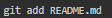
\includegraphics[width=0.5\linewidth]{add.png}
	\end{minipage}
	
	7.展示历来提交版本:git log
	
	\noindent
	\begin{minipage}{\linewidth}
		\centering
		% 插入图片
		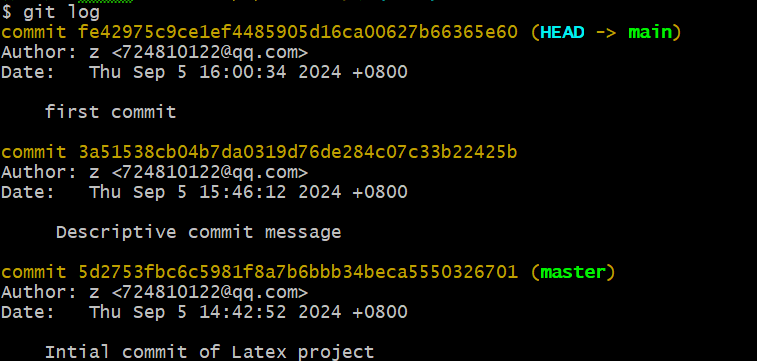
\includegraphics[width=0.5\linewidth]{log.png}
	\end{minipage}
	
	8.打开任意版本:git show hash
	
	\noindent
	\begin{minipage}{\linewidth}
		\centering
		% 插入图片
		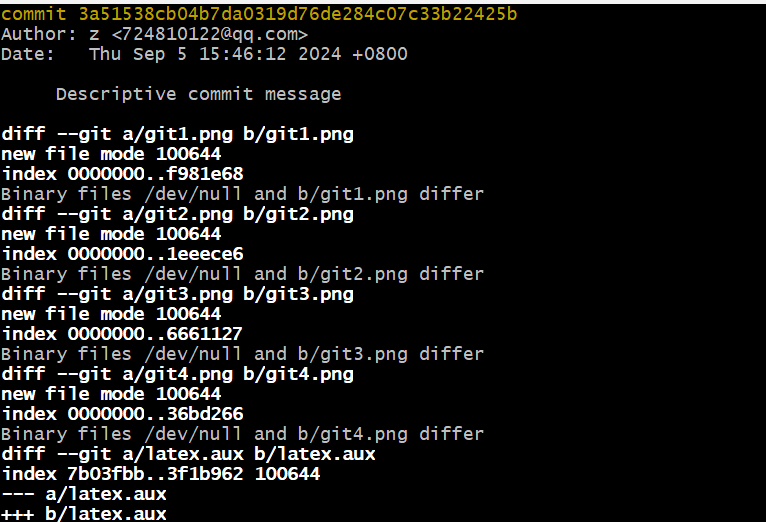
\includegraphics[width=0.5\linewidth]{hash.png}
	\end{minipage}
	
	9. 将当前分支回退到指定的提交:git reset --hard [commit hash]
	
	不做演示
	
	10.查看工作目录和暂存区之间的差异:git diff
	
	\noindent
	\begin{minipage}{\linewidth}
		\centering
		% 插入图片
		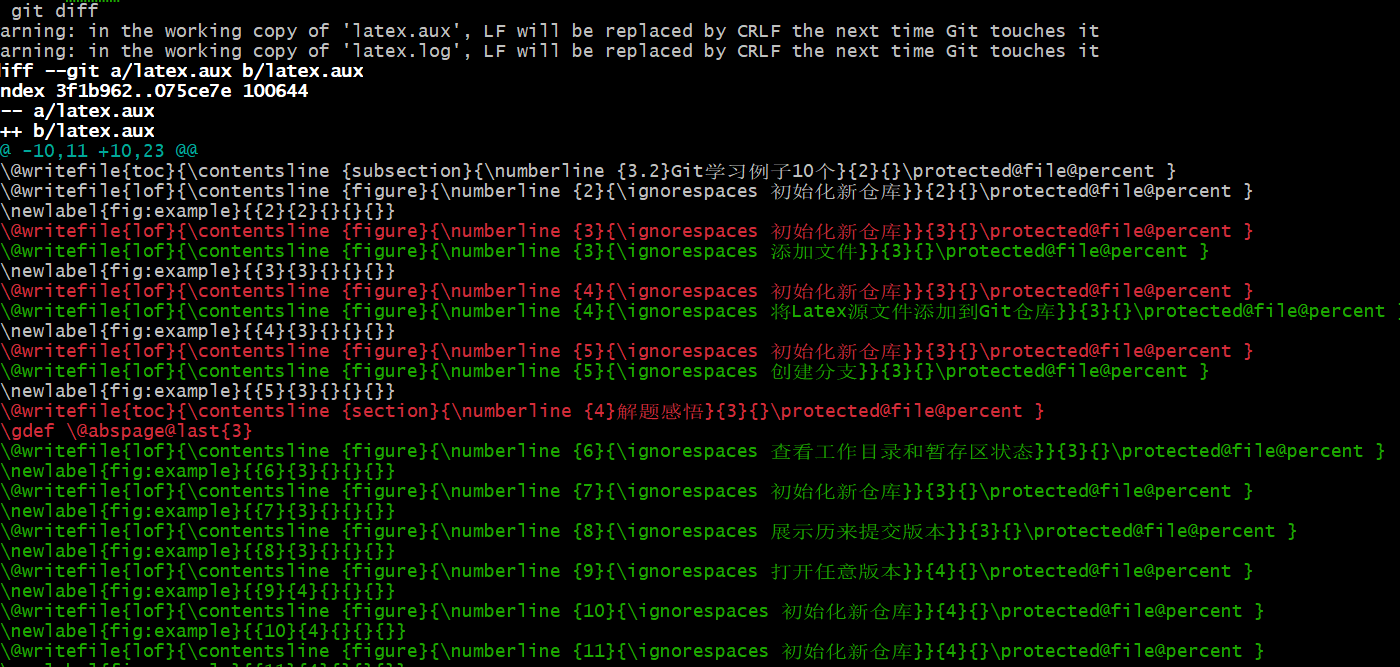
\includegraphics[width=0.5\linewidth]{diff.png}

	\end{minipage}
	
	
	
	
	\section{解题感悟}
	通过学习LaTeX,我学会了如何制作出格式严谨的文档。在撰写实验报告时,我可以更专注于内容的编写,而不是文档的格式调整。
	
	git具有良好的branch机制,这样可以让主干代码保持干净,对于大型项目来说非常不错。
	
	github路径
	您可以在此查看项目的源代码: 
	
	\url{https://github.com/L-c-hang/xuexi}
	

\end{document}
